\section{DecMed}
\label{sec:decmed}

Sistem DecMed adalah sebuah kerangka kerja manajemen RME terdesentralisasi yang dibangun di atas DLT IOTA \autocite{sadewa2025decmed}. Pengembangan sistem ini bertujuan untuk mengatasi tantangan fragmentasi data antarinstitusi kesehatan dan risiko keamanan dari penyimpanan terpusat yang ada di Indonesia.

\subsection{Arsitektur DecMed}
\label{subsec:arsitektur-decmed}

Arsitektur DecMed membagi penyimpanan menjadi dua lapisan, yaitu penyimpanan \textit{on-chain} dan \textit{off-chain}. Penyimpanan \textit{off-chain} memanfaatkan IPFS untuk menyimpan data klinis pasien yang terenkripsi. Sementara itu, penyimpanan \textit{on-chain} memanfaatkan DLT IOTA untuk menyimpan data administratif dan metadata klinis, termasuk CID dari IPFS, guna menjamin integritas data. Untuk memastikan kedaulatan data pasien, DecMed mengimplementasikan CapBAC yang diintegrasikan dengan PRE. Skema PRE yang diterapkan pada DecMed adalah Umbral PRE yang dijelaskan pada Subbab \ref{subsec:umbral-pre}. Gambar~\ref{fig:decmed-archi} merangkum hubungan komponen tersebut.

\begin{figure}[htbp]
	\centering
	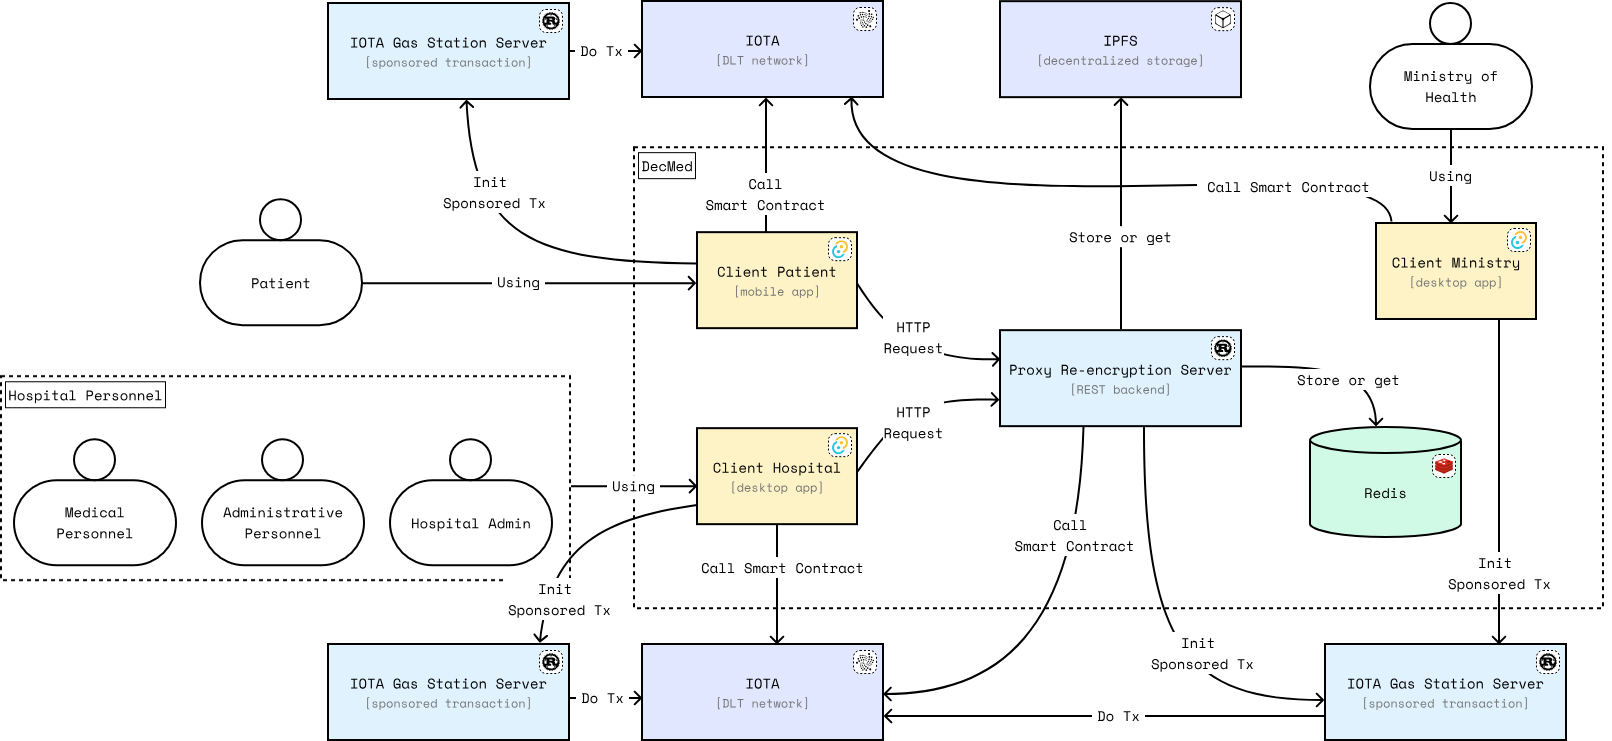
\includegraphics[width=1\textwidth]{resources/chapter-2/decmed_archi.png}
	\caption{Arsitektur DecMed \autocite{sadewa2025decmed}.}
	\label{fig:decmed-archi}
\end{figure}

Gambar~\ref{fig:decmed-archi} menunjukkan pemisahan penyimpanan metadata pada IOTA dan data terenkripsi pada IPFS, dengan PRE sebagai titik verifikasi dan \textit{re-encryption} sebelum data dibuka oleh penerima akses. Peran tiap komponen dan aktor dirinci pada Tabel~\ref{tab:decmed-komponen}.

\begin{table}[htbp]
	\centering
	\caption{Komponen, aktor, dan fungsi dalam arsitektur DecMed}
	\label{tab:decmed-komponen}
	\begin{tabularx}{\textwidth}{|>{\raggedright\arraybackslash}p{0.26\textwidth}|>{\raggedright\arraybackslash}X|}
		\hline
		\textbf{Komponen / Aktor} & \textbf{Fungsi}                                                                                                                                                    \\
		\hline
		IOTA DLT                  & Menyimpan metadata, referensi data, dan status akses                                                                                                               \\
		\hline
		IPFS                      & Menyimpan \textit{encrypted blob} data RME                                                                                                                         \\
		\hline
		PRE                       & Melakukan verifikasi token akses dan \textit{re-encryption} agar penerima akses dapat membuka data tanpa kunci privat pasien                                       \\
		\hline
		Redis                     & Mengelola \textit{cache ephemeral} (\texttt{Nonce}, \texttt{Re-Encryption Key}, dan \texttt{Revoked Key})
		\\
		\hline
		\textit{Patient Client}   & Digunakan pasien untuk mengelola identitas, menyimpan atau memperbarui data, serta memberi akses                                                                   \\
		\hline
		\textit{Hospital Client}  & Digunakan tenaga kesehatan / fasyankes untuk mengakses atau memperbarui RME sesuai hak akses                                                                       \\
		\hline
		\textit{Ministry Client}  & Digunakan pemerintah untuk mengelola registrasi atau verifikasi fasyankes                                                                                          \\
		\hline
		\textit{IOTA Gas Station} & Mensponsori transaksi \textit{on-chain} agar pengguna tidak perlu membayar \textit{gas} secara langsung; pada Tugas Akhir ini diasumsikan sebagai bagian dari IOTA \\
		\hline
	\end{tabularx}
\end{table}

Tabel~\ref{tab:decmed-komponen} menegaskan bahwa DecMed memisahkan peran penyimpanan, penegakan akses, dan antarmuka aktor: IOTA dan IPFS tidak menyimpan \textit{plaintext} klinis, sedangkan ketiga \textit{client} merepresentasikan kepentingan pasien, fasyankes, dan pemerintah.

\subsection{Alur Pengelolaan dan Akses RME pada DecMed}

Alur pengelolaan RME pada DecMed dimulai ketika data medis dibuat melalui aplikasi \textit{hospital client}. Data tersebut dienkripsi terlebih dahulu di sisi \textit{client} sebelum disimpan pada IPFS. Setelah data terenkripsi berhasil diunggah, IPFS menghasilkan CID sebagai referensi lokasi data. CID, \textit{capsule key}, dan metadata pendukung kemudian dicatat pada DLT IOTA. Dengan demikian, IOTA tidak menyimpan isi rekam medis secara langsung, melainkan menyimpan metadata yang diperlukan untuk menemukan, memverifikasi, dan membuka data terenkripsi melalui mekanisme PRE.

Ketika pasien memberikan akses kepada tenaga kesehatan, PRE menerbitkan token kapabilitas yang digunakan sebagai bukti otorisasi. Penerima akses membawa token tersebut ketika meminta data melalui \textit{Hospital Client}. \textit{Server} PRE kemudian memverifikasi token, melakukan \textit{re-encryption} terhadap \textit{capsule key}, dan mengembalikan material kriptografis yang diperlukan agar \textit{Hospital Client} dapat membuka data terenkripsi sesuai hak akses yang diberikan. \textit{Sequence Diagram} yang menjelaskan alur pemberian akses dapat dilihat pada Lampiran \ref{lampiran:alur-pemberian-akses-medis}.
